%% Source: https://github.com/tias/constraint-solving-course
%% Licensed under CC BY-NC-SA 4.0: https://creativecommons.org/licenses/by-nc-sa/4.0/
%% You may share and adapt this for non-commercial use,
%% with attribution and under the same license.

\documentclass{cons-beamer}

\begin{document}


\begin{frame}{L05: Viewpoints and redundant constraints}
  \begin{center}
    ~ \\
    \includegraphics[height=35mm]{images/ssp.png} \\
    Prof. Tias Guns and Dr. Dimos Tsouros \\[0.5em]
    \includegraphics[width=2cm]{images/kuleuven_CMYK_logo.pdf}
  \end{center}
  
  {\footnotesize 
  Partly based on slides from Pierre Flener and Barbara Smith.}
  % https://pierre-flener.github.io/courses/M4CO/lectures.html
\end{frame}

\begin{frame}{Quick Recap}
  \begin{enumerate}
    \item \inference{Modelling}: express problem in terms of \vfill
    \begin{itemize}
      \item parameters, \vfill
      \item decision variables, with their domains \vfill
      \item constraints, and \vfill
      \item (optionally) objective.
    \end{itemize} \vfill
    \item \search{Solving}: solve using a state-of-the-art solver.
  \end{enumerate}
\end{frame}

\begin{frame}{A Modelling Methodology: Overview}
  \raisebox{-\height}[0pt][0pt]{%
    \begin{columns}
      \begin{column}{0.7\textwidth}
          
      \end{column}
      \begin{column}{0.3\textwidth}
        \includegraphics[height=38mm]{images/how_to_model.png}%
      \end{column}
    \end{columns}
  }

  \begin{enumerate}
    \item Make sure you understand the problem correctly:
    \begin{itemize}
      \item Find out what is given and what is unknown \\$\xrightarrow{}$ what needs to be decided.
      \item Find out what the objective is, if any.
    \end{itemize}
    \vfill
    \item Construct or select some small instance(s) \\of your problem to work with.
    \vfill
    \item Model incrementally: 
    \begin{itemize}
      \item Add a constraint at a time and verify that it is correct.
      \item Only add the objective function, if any, at the end.
    \end{itemize}
    \vfill
    \item Model first for correctness and clearness, then for efficiency:
    \begin{itemize}
      \item Try to use predefined predicates when relevant.
      \item Once you have a correct model, consider symmetries and redundant constraints.
      \item Only as a last resort, add annotations.
    \end{itemize}
    %\item Experiment with different models and different solvers.
  \end{enumerate}
\end{frame}


\section{Viewpoints}

\begin{frame}{What is a good model for a constraint problem?}
  You get the problem definition of a constraint problem. \vfill 
  \begin{itemize}
    \item You now have to model it \blue{correctly} (and \inference{efficiently})!
  \end{itemize}
  \vfill 

  How do you choose which of the entities of the problem are the decision variables?
  \vfill 

  \begin{example}[Task allocation]
    There are three workers (W1, W2, W3). Our current project has 4 tasks that have to be allocated to a worker: Construct Product (CP) and Quality Check (QC), which will be conducted on Thursday, and Package Product (PP) and Transport Product (TP), which will be conducted on Friday. No worker should handle two tasks on the same day.  Worker W3 cannot work this on Thursday. Worker W1 can only perform tasks QC and TP.
  \end{example}
\end{frame}

\begin{frame}{Viewpoints}
  Different models of a problem may result from viewing the problem from different angles or perspectives, i.e. different \defined{viewpoints}.
  \vfill

  The \defined{viewpoint} defines the variables and domains of your model.
  \vfill

  \begin{definition}[Law and Lee, 2002]
    A \defined{viewpoint} is a pair \(\langle X, D \rangle\), where \(X = \{x_1, \ldots, x_n\}\) is a set of variables, and \(D\) is a set of domains. For each \(x_i \in X\), the associated domain \(D_i\) is the set of possible values for \(x_i\). It must be possible to ascribe a meaning to the variables and values of the CSP in terms of the problem \(P\), and so to say what an assignment in the viewpoint \(\langle X, D \rangle\) is intended to represent in terms of \(P\).
  \end{definition}
  \vfill

  \alert{Based on the chosen viewpoint, the size of the search space changes}
\end{frame}

\begin{frame}{Viewpoints and size of the search space }

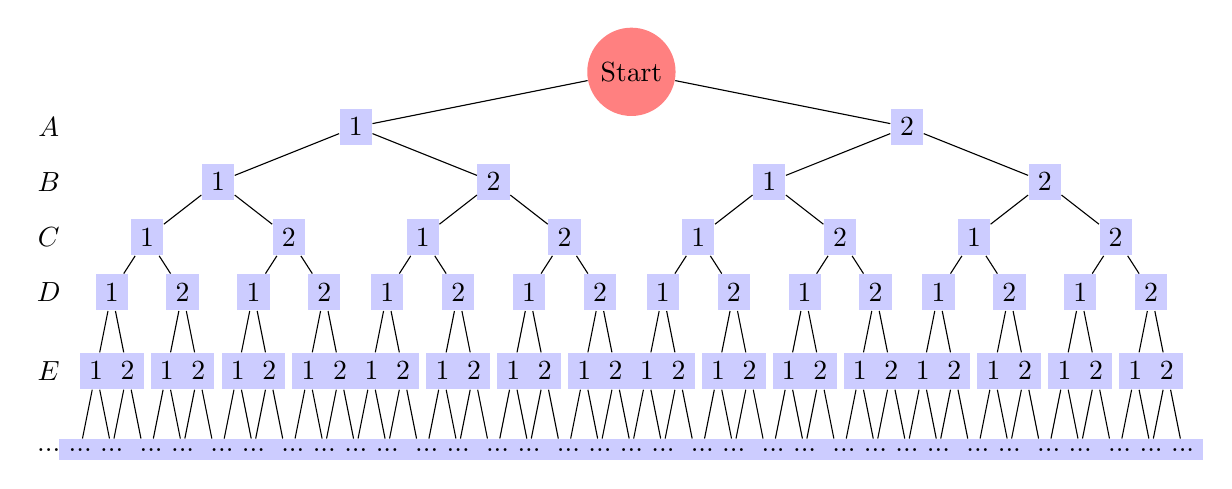
\begin{tikzpicture}[
val/.style={rectangle, fill=blue!20},
root/.style={circle, fill=red!50},
var/.style={rectangle},
level 1/.style={level distance=0.7cm, sibling distance=7cm},
level 2/.style={level distance=0.7cm, sibling distance=3.5cm},
level 3/.style={level distance=0.7cm, sibling distance=1.8cm},
level 4/.style={level distance=0.7cm, sibling distance=0.9cm},
level 5/.style={level distance=1cm, sibling distance=0.4cm},
]

% Variables listed on the side
\coordinate (V) at (-7.4,0);
\node[var] at (V) { };
\coordinate (A) at (-7.4,-0.7);
\node[var] at (A) {$A$};
\coordinate (B) at (-7.4,-1.4);
\node[var] at (B) {$B$};
\coordinate (C) at (-7.4,-2.1);
\node[var] at (C) {$C$};
\coordinate (D) at (-7.4,-2.8);
\node[var] at (D) {$D$};
\coordinate (E) at (-7.4,-3.8);
\node[var] at (E) {$E$};
\coordinate (E) at (-7.4,-4.8);
\node[var] at (E) {...};

% Root node and expanded search space with values only
\node[root] {Start} 
  child{node[val]{1} % A=1
    child{node[val]{1} % B=1
      child{node[val]{1} % C=1
        child{node[val]{1} % D=1
          child{node[val]{1}
           child{node[val]{...}}
           child{node[val]{...}}           
           } % E=1
          child{node[val]{2}
           child{node[val]{...}}
           child{node[val]{...}}  
           } % E=2
        }
        child{node[val]{2} % D=2
          child{node[val]{1}
         child{node[val]{...}}
           child{node[val]{...}}
           } % E=1
          child{node[val]{2}
           child{node[val]{...}}
           child{node[val]{...}}  
           } % E=2
        }
      }
      child{node[val]{2} % C=2
        child{node[val]{1} % D=1
          child{node[val]{1}
           child{node[val]{...}}
           child{node[val]{...}}           
           } % E=1
          child{node[val]{2}
           child{node[val]{...}}
           child{node[val]{...}}  
           } % E=2
        }
        child{node[val]{2} % D=2
          child{node[val]{1}
           child{node[val]{...}}
           child{node[val]{...}}           
           } % E=1
          child{node[val]{2}
           child{node[val]{...}}
           child{node[val]{...}}  
           } % E=2
        }
      }
    }
    child{node[val]{2} % B=2
      child{node[val]{1} % C=1
        child{node[val]{1} % D=1
          child{node[val]{1}
           child{node[val]{...}}
           child{node[val]{...}}           
           } % E=1
          child{node[val]{2}
           child{node[val]{...}}
           child{node[val]{...}}  
           } % E=2
        }
        child{node[val]{2} % D=2
          child{node[val]{1}
           child{node[val]{...}}
           child{node[val]{...}}           
           } % E=1
          child{node[val]{2}
           child{node[val]{...}}
           child{node[val]{...}}  
           } % E=2
        }
      }
      child{node[val]{2} % C=2
        child{node[val]{1} % D=1
          child{node[val]{1}
           child{node[val]{...}}
           child{node[val]{...}}           
           } % E=1
          child{node[val]{2}
           child{node[val]{...}}
           child{node[val]{...}}  
           } % E=2
        }
        child{node[val]{2} % D=2
          child{node[val]{1}
           child{node[val]{...}}
           child{node[val]{...}}           
           } % E=1
          child{node[val]{2}
           child{node[val]{...}}
           child{node[val]{...}}  
           } % E=2
        }
      }
    }
  }
  child{node[val]{2} % A=2
    child{node[val]{1} % B=1
      child{node[val]{1} % C=1
        child{node[val]{1} % D=1
          child{node[val]{1}
           child{node[val]{...}}
           child{node[val]{...}}           
           } % E=1
          child{node[val]{2}
           child{node[val]{...}}
           child{node[val]{...}}  
           } % E=2
        }
        child{node[val]{2} % D=2
          child{node[val]{1}
           child{node[val]{...}}
           child{node[val]{...}}           
           } % E=1
          child{node[val]{2}
           child{node[val]{...}}
           child{node[val]{...}}  
           } % E=2
        }
      }
      child{node[val]{2} % C=2
        child{node[val]{1} % D=1
          child{node[val]{1}
           child{node[val]{...}}
           child{node[val]{...}}           
           } % E=1
          child{node[val]{2}
           child{node[val]{...}}
           child{node[val]{...}}  
           } % E=2
        }
        child{node[val]{2} % D=2
          child{node[val]{1}
           child{node[val]{...}}
           child{node[val]{...}}           
           } % E=1
          child{node[val]{2}
           child{node[val]{...}}
           child{node[val]{...}}  
           } % E=2
        }
      }
    }
    child{node[val]{2} % B=2
      child{node[val]{1} % C=1
        child{node[val]{1} % D=1
          child{node[val]{1}
           child{node[val]{...}}
           child{node[val]{...}}           
           } % E=1
          child{node[val]{2}
           child{node[val]{...}}
           child{node[val]{...}}  
           } % E=2
        }
        child{node[val]{2} % D=2
          child{node[val]{1}
           child{node[val]{...}}
           child{node[val]{...}}           
           } % E=1
          child{node[val]{2}
           child{node[val]{...}}
           child{node[val]{...}}  
           } % E=2
        }
      }
      child{node[val]{2} % C=2
        child{node[val]{1} % D=1
          child{node[val]{1}
           child{node[val]{...}}
           child{node[val]{...}}           
           } % E=1
          child{node[val]{2}
           child{node[val]{...}}
           child{node[val]{...}}  
           } % E=2
        }
        child{node[val]{2} % D=2
          child{node[val]{1}
           child{node[val]{...}}
           child{node[val]{...}}           
           } % E=1
          child{node[val]{2}
           child{node[val]{...}}
           child{node[val]{...}}  
           } % E=2
        }
      }
    }
  };

\end{tikzpicture}


  Search space has breadth $d$ and depth $n$, with $d$ being the size of the domains, and $n$ the amount of decision variables used: \textbf{$d^n$ leaves = complete assignments}
    
\end{frame}

\begin{frame}{What is a good model for a constraint problem?}
  \begin{example}[Task allocation]
    \begin{center}
      \includegraphics[height=30mm]{images/task_allocation.png}
    \end{center}

    There are three workers (W1, W2, W3). Our current project has 4 tasks that have to be allocated to a worker: Construct Product (CP) and Quality Check (QC), which will be conducted on Thursday, and Package Product (PP) and Transport Product (TP), which will be conducted on Friday. No worker should handle two tasks on the same day.  Worker W3 cannot work this Thursday. Worker W1 can only perform tasks QC and TP.
  \end{example}
\end{frame}

\begin{frame}{What is a good model for a constraint problem?}
    \begin{example}[Task allocation]
      There are three workers (W1, W2, W3). Our current project has 4 tasks that have to be allocated to a worker: Construct Product (CP) and Quality Check (QC), which will be conducted on Thursday, and Package Product (PP) and Transport Product (TP), which will be conducted on Friday. No worker should handle two tasks on the same day.  Worker W3 cannot work this Thursday. Worker W1 can only perform tasks QC and TP.
    \end{example}

    We have 2 types of entities: the workers $\{W1, W2, W3\}$ and the tasks $\{CP, QC, PP, TP\}$. Which are my variables?\vfill
    \begin{enumerate}
      \item \defined{Viewpoint} 1: Workers as variables $\xrightarrow{}$ Which task(s) is assigned to each worker?\vfill
      \item \defined{Viewpoint} 2: Tasks as variables $\xrightarrow{}$ Which worker is each task assigned to?\vfill
    \end{enumerate}
\end{frame}

\begin{frame}{Workers as variables}
  \textbf{Decision Variables}
  One for each worker, so we have 3 variables: W1, W2 and W3
  \vfill

  \textbf{Initial Domains} The workers are 3 and the tasks are 4. So, each worker has to be assigned one or more shifts, to have all tasks allocated, meaning that there must be (at least) one worker that will have 2 task. 
  \vfill

  So, the domains will be all tasks, but also all pairs of them: 
  $\{\{CP\}, \{QC\}, \{PP\}, \{TP\}, \{CP, QC\}, \{CP, PP\}, \{CP, TP\}, \allowbreak \{QC, PP\}, \{QC, TP\}, \{PP, TP\}\}$
  \vfill

  Size of the \search{search space}?
  

  Domains of size $10$, and $3$ variables: $10^3 = 1000$ candidate solutions.
  \vfill

  \textbf{Constraints} All tasks have to be assigned to only one worker. Can we represent it with just pairwise, not equal constraints?  \alert{No}. \\ \alert{Also, too many unary constraints to model each restriction of the workers.}
\end{frame}

\begin{frame}{Tasks are variables}
  \textbf{Decision Variables}
  One for each shift, so we have 4 variables: $\{CP, QC, PP, TP\}$
  \vfill

  \textbf{Initial Domains} Each task has to be assigned to a worker. So, the initial domain of every decision variable is the set of workers: $\{W1, W2, W3\}$.
  \vfill

  \textcolor{red}{The problem representation is much easier even before formulating the constraints! The initial domains are much more straightforward}
  \vfill

  Size of the \search{search space}?
  

  Domains of size $3$, and $4$ variables: $3^4 = 81$ candidate solutions.
\end{frame}

\begin{frame}{Tasks are variables}
  \textbf{Constraints} Each task has to be assigned to a worker. No constraints are needed to represent that now. Let's model the unary constraints:
  \vfill

  \begin{enumerate}
    \item No worker should be assigned two tasks in the same day:
          \begin{itemize}
            \item $CP \neq QC$
            \item $PP \neq TP$
          \end{itemize}
          \vfill

    \item Worker W3 cannot work this Thursday. 
          \begin{itemize}
            \item $CP \neq W3$
            \item $QC \neq W3$
          \end{itemize}
          \vfill

    \item Worker W1 can only perform tasks QC and TP. 
          \begin{itemize}
            \item $CP \neq W1$
            \item $PP \neq W1$
          \end{itemize}
  \end{enumerate}
\end{frame}

\begin{frame}{Viewpoints}
  Choosing the right viewpoint can make modeling way easier.
  \vfill

  Ease of formulating constraints and (optionally) the objective function: Important on choosing the viewpoint to use.
  \vfill

  \begin{itemize}
    \item Typically leads also to better \textbf{readability!}
    \item This may be very important, depending on the user of the model and their background \dots
  \end{itemize}
  \vfill

  \alert{But is one viewpoint always clearly the right one to use?}
\end{frame}

\begin{frame}[t]\label{studSeat}
  \begin{example}[Student Seating Problem]
    \begin{minipage}[c]{0.33\linewidth}
      \includegraphics[width=\linewidth]{images/ssp} \\
      \tiny
      $\mathtt{nStudents} = \red{15}$ \\ $\mathtt{nPgms} = 3$ \\
      $\mathtt{nChairs} = \blue{20} \geq \mathtt{nStudents}$ \\
      $\mathtt{nTables} = 5$ \\
      $\mathtt{Chairs} = [1..4,5..8,9..12,13..16,17..20]$
    \end{minipage}
    \hfill
    \begin{minipage}[c]{0.66\linewidth}
      Given:
      \begin{itemize}
        \item $\mathtt{nStudents}$ students,
        \item $\mathtt{nPgms}$ study programmes
        \item $\mathtt{nChairs}$ chairs around $\mathtt{nTables}$ tables, and
        \item $\mathtt{Chairs[t]}$ as the set of chairs of table $\mathtt{t}$,
      \end{itemize}
      \vfill

      Find a seating arrangement such that:
      \begin{enumerate}
        \item each table has students of distinct study programmes;
        \item each table has either at least half or none of its chairs occupied;
        \item a maximum number of student preferences on being seated at the same table are satisfied.
      \end{enumerate}
    \end{minipage}
  \end{example}\vfill
 \vfill
  What are suitable decision variables for this problem?
\end{frame}

\begin{frame}
  A \defined{viewpoint} is a choice of decision variables.
  \vfill

  \begin{example}[Student Seating Problem]
    \structured{Viewpoint 1:}  Which chair does each student sit on?
    
    Variables represent the students, domains represent the chairs they will sit on.
    \footnotesize
    \[ \mathtt{student}_s \in \{1, \ldots, \mathtt{nChairs}\}, \quad \forall s \in \{1, \ldots, \mathtt{nStudents}\} \]
    \[ \cons{AllDifferent}{\mathtt{student}} \]
    \normalsize
     \vfill

    \structured{Viewpoint 2:}  Which student, if any, sits on each chair?

    Variables represent the chairs, domains represent the students that will sit on them.
    
    \footnotesize
    \[ \mathtt{chair}_c \in \{0, \ldots, \mathtt{nStudents}\}, \quad \forall s \in \{1, \ldots, \mathtt{nChairs}\} \]
    \[ \cons{AllDifferentExceptN}{\mathtt{chair}, 0} \]
    \normalsize
    \vfill

    \alert{Notice that we use student $0$ to represent that no student is sitting on that chair \dots}

    It does not need to be a $0$, but a \defined{dummy value}. Depending on the problem, we may have several \defined{dummy values}
  \end{example}\vfill
\end{frame}

\begin{flashcardcpmpy}
\begin{frame}
  A \defined{viewpoint} is a choice of decision variables.
  \vfill

  \begin{example}[Student Seating Problem -- CPMpy]
    \structured{Viewpoint 1:}  Which chair does each student sit on?
    
    Variables represent the students, domains represent the chairs they will sit on.
    \footnotesize
    \lstinputlisting[language=cpmpy,firstline=12,lastline=13,numbers=none]{models_cpmpy/t5_student_seating.py}
    \normalsize
     \vfill

    \structured{Viewpoint 2:}  Which student, if any, sits on each chair?

    Variables represent the chairs, domains represent the students that will sit on them.
    
    \footnotesize
    \lstinputlisting[language=cpmpy,firstline=16,lastline=17,numbers=none]{models_cpmpy/t5_student_seating.py}
    \normalsize
    \vfill

    \alert{Notice that we use student $0$ to represent that no student is sitting on that chair \dots}

    It does not need to be a $0$, but a \defined{dummy value}. Depending on the problem, we may have several \defined{dummy values}
  \end{example}\vfill
\end{frame}
\end{flashcardcpmpy}

\begin{frame}
  Different \defined{viewpoints} offer different advantages and disadvantages.

  \begin{itemize}
    \item Ease of formulating the constraints and (optionally) the objective (as discussed).
    \begin{itemize}
      \item It depends on the unstated other constraints.
      \item Ideally, we want a viewpoint that allows global constraints to be used.
    \end{itemize}
    

    \item Readability. 
      \begin{itemize}
        \item Who is going to read the model, and what is their background?
      \end{itemize}
      
    \item Size of the search space. 
      \begin{itemize}
        \item Viewpoint 1: $\Oh{\mathtt{nChairs}^{\mathtt{nStudents}}}$
        \item Viewpoint 2: $\Oh{(\mathtt{nStudents} + 1)^{\mathtt{nChairs}}}$
      \end{itemize} 
    
    \item Performance:
      \begin{itemize}
        \item The size is not the only factor for the performance
        \item In general, \red{hard} to tell: we have to run experiments!
      \end{itemize}
  \end{itemize}
  

  \alert{Typically, there is no one correct answer here: \\ when in doubt: run comparative experiments.}
\end{frame}


\section{Auxiliary variables}

\begin{frame}{Auxiliary variables}
  \begin{definition}
    \defined{Auxiliary variables} are variables that are introduced in the model during the modeling process, and are not necessary related to entities of our problem.
  \end{definition}
  \vfill

  Auxiliary variables may be necessary:
  \begin{itemize}
    \item You may not be able to express certain constraints directly using the variables of the chosen \textit{viewpoint}
    \item Depending on the used \textit{solving technology/language}, auxiliary variables may need to be introduced to allow the specification of higher arity constraints.
  \end{itemize}
  \vfill

  Auxiliary variables may be useful:
  \begin{itemize}
    \item Expressing constraints may be \textit{easier} using auxiliary variables.
    \item Resulting model may be more \textit{readable}.
    \item Propagation of constraints may be more \textit{efficient}.
  \end{itemize}
\end{frame}

\begin{frame}{Auxiliary variables}
  \begin{example}[Car Sequencing; Dincbas, Simonis and van Hentenryck, 1988]
    \begin{columns}
      \begin{column}{0.35\textwidth}
        \begin{itemize}
          \item 10 cars to be made on a production line, each requires some options
          \item Stations installing options have lower capacity than rest of line e.g. at most 1 car out of 2 for option 1
          \item Find a feasible production sequence
        \end{itemize}
      \end{column}
      \begin{column}{0.6\textwidth}
        \begin{center}
          \begin{tabular}{|c|c|c|c|c|c|c|c|}
            \hline
            \textbf{Classes} & \textbf{1} & \textbf{2} & \textbf{3} & \textbf{4} & \textbf{5} & \textbf{6} & \textbf{Capacity} \\
            \hline
            \textbf{Option 1} & 1 & 0 & 0 & 0 & 1 & 1 & 1/2 \\
            \hline
            \textbf{Option 2} & 0 & 0 & 1 & 1 & 0 & 1 & 2/3 \\
            \hline
            \textbf{Option 3} & 1 & 0 & 0 & 0 & 1 & 0 & 1/3 \\
            \hline
            \textbf{Option 4} & 1 & 1 & 0 & 1 & 0 & 0 & 2/5 \\
            \hline
            \textbf{Option 5} & 0 & 0 & 1 & 0 & 0 & 0 & 1/5 \\
            \hline
            \textbf{No. of cars} & 1 & 1 & 2 & 2 & 2 & 2 & \\
            \hline
          \end{tabular}
        \end{center}
      \end{column}    
    \end{columns}
  \end{example}
\end{frame}


\begin{frame}{Auxiliary variables - Car Sequencing}
  % Add the image at the top right corner
  \raisebox{-\height}[0pt][0pt]{%
    \begin{columns}
      \begin{column}{0.7\textwidth}
          
      \end{column}
      \begin{column}{0.3\textwidth}
        \includegraphics[height=35mm]{images/car_seq.png}%
      \end{column}
    \end{columns}
  }

  \begin{itemize}
    \item Viewpoint:
      \begin{itemize}
        \item A variable for each position in the sequence, \\
        \(s_1, s_2, \ldots, s_{10} \in S\)

        \item Value of \(s_i\) is the class of car in position \(i\)
      \end{itemize}
      \vfill
    
    \item Constraints:
      \begin{itemize}
        \item Each class occurs the correct number of times
        \[ CountEq(s, k, d_k) \quad \forall k \in \mathtt{Classes} \]
        with $d_k$ being the production demand for class $k$.  \inference{Or better}:

        \[ GlobalCardinalityCount(S, Classes, D) \]
        with $D$ being the list of production demands for each class.
        \vfill

        \item Option capacities are respected - ?
      \end{itemize}
  \end{itemize}    

  \vfill
  \alert{Cannot model the option capacities directly by using variables $s_i$!  (Actually we can, with a long and complex constraint that will create auxiliary variables either way)}
  \vfill
\end{frame}


\begin{frame}{Auxiliary variables - Car Sequencing}
  % Add the image at the top right corner
  \raisebox{-\height}[0pt][0pt]{%
    \begin{columns}
      \begin{column}{0.7\textwidth}
            
      \end{column}
      \begin{column}{0.3\textwidth}
        \includegraphics[height=35mm]{images/car_seq.png}%
      \end{column}
    \end{columns}
  }

  How can we model the constraints for the option capacities?
  \vfill

  \begin{itemize}
    \item Introduce \defined{auxiliary} variables \(o_{ij}\):
      \begin{itemize}
        \item \(o_{ij} = 1\) iff the car in the \(i\)-th slot in the sequence requires option \(j\)
      \end{itemize}
      \vfill

    \item \textit{Constraints}, e.g. option 1 capacity is one car in every two:
      \begin{itemize}
        \item \(o_{i,1} + o_{i+1,1} \leq 1 \quad \text{for} \quad 1 \leq i < 10\)
      \end{itemize}
      \vfill

    \item Relate the auxiliary variables to the \(s_i\) variables:
      \begin{itemize}
        \item Matrix \(\lambda_{jk} = 1\) representing if car class \(k\) requires option \(j\)
        \item \(o_{ij} = \lambda_{js_i} \quad 1 \leq i \leq 10, \, 1 \leq j \leq 5\) 
              $\xrightarrow{}$ \alert{Reminder: This uses in practice the \texttt{Element} constraint. A variable ($s_i$) is used as index in an array.}
      \end{itemize}
  \end{itemize}
\end{frame}

\begin{flashcardcpmpy}
\begin{frame}{Auxiliary variables -- Car Sequencing -- CPMpy}
  \begin{example}[CPMpy model for Car Sequencing]
    \lstinputlisting[language=cpmpy,basicstyle=\scriptsize,numbers=none,firstline=13,lastline=29]{models_cpmpy/car_sequencing.py}
  \end{example}
\end{frame}
\end{flashcardcpmpy}


\section{Redundant Constraints}

\begin{frame}{Redundant constraints}
  We have chosen a viewpoint, and formulated the constraints to solve our problem \blue{correctly}. But, can we do something to make it more \inference{efficient}?
  \vfill

  During the search process, the solver will explore several infeasible parts of the search tree. Can we avoid that?
  \vfill

  \begin{definition}
    \defined{Redundant constraints}, also called \textit{implied} constraints, are constraints which are entailed by the constraints defining the problem. They do not change the set of solutions, and hence are logically redundant.
  \end{definition}
  \vfill

  Although \defined{redundant} constraints are logically redundant, and do not change the set of solutions, they can be used to \blue{reduce the search effort of the solving process}. 
\end{frame}

\begin{frame}{Redundant constraints}
  \begin{definition}
  	\defined{Redundant constraints}, also called \textit{implied} constraints, are constraints which are entailed by the constraints defining the problem. They do not change the set of solutions, and hence are logically redundant.
  \end{definition}
  \vfill

  Redundant constraints are often added to the model to reduce the search effort, by \red{cutting infeasible parts} of the search tree early. 
  So the solver does not need to explore possible assignments in these subproblems \dots   
  \vfill

  \begin{itemize}
    \item at some point during search, we will have a partial assignment that cannot lead to a solution
    \item the redundant constraint can detect inconsistency of the partial assignment
          \begin{itemize}
            \item the redundant constraint forbids it, but \textbf{does not change the set of solutions}
          \end{itemize}
    \item while without the redundant constraint, the search would continue deeper
  \end{itemize}
\end{frame}

\begin{frame}{Redundant constraints -- Car Sequencing}
  % Add the image at the top right corner
  \raisebox{-\height}[0pt][0pt]{%
    \begin{columns}
      \begin{column}{0.7\textwidth}
          
      \end{column}
      \begin{column}{0.3\textwidth}
        \includegraphics[height=35mm]{images/car_seq.png}%
      \end{column}
    \end{columns}
  }

  \begin{itemize}
      \item Existing constraints only say that the option capacities \\ cannot be \emph{exceeded}
            \begin{itemize}
                \item but we can’t stay too far below capacity either
            \end{itemize}
            \vfill

      \item Suppose there are 30 cars, and 12 require option 1 
      \vfill
      
      \item Reminder: Option 1 capacity is 1 car in 2
      \vfill

      \item At least one car in slots 1 to 8 of the production sequence \\ must have option 1
            \begin{itemize}
              \item otherwise 12 of cars 9 to 30 will require option 1, i.e. too many
            \end{itemize}
      \vfill

      \item Cars 1 to 10 must include at least two option 1 cars, \ldots, and cars 1 to 28 must include at least 11 option 1 cars
      \vfill

      \item These are \emph{implied constraints} that can be used to speed up search in car sequencing
  \end{itemize}
\end{frame}

\begin{frame}
  \begin{example}[Magic Series of length \texttt{n}]
    The element at index \texttt{i} in \texttt{I = 0..(n-1)} is
    the number of occurrences of \texttt{i}.  Solutions:
    $\mathtt{Magic}=[1,2,1,0]$ and
    $\mathtt{Magic}=[2,0,2,0]$ for $\mathtt{n}=4$. \\~\\

    \structured{Decision variables:}
    

    \texttt{Magic} ~=~
    \begin{tabular}{cccc}
      \texttt{0} & \texttt{1} & $\cdots$ & \texttt{n-1} \\
      \hline
      \multicolumn{1}{|c|}{$\in \mathtt{I}$} &
      \multicolumn{1}{|c|}{$\in \mathtt{I}$} &
      \multicolumn{1}{|c|}{$\cdots$} &
      \multicolumn{1}{|c|}{$\in \mathtt{I}$} \\
      \hline
    \end{tabular} \\~\\ 

	\small
    \structured{Problem Constraint:}
    \[ \forall i \in I, \quad \text{Magic}[i] = \sum_{j \in I} (\text{Magic}[j] = i) \] 
    or, logically equivalently but better:
    \[ \forall i \in I, \quad \text{CountEq}(\text{Magic}, i, \text{Magic}[i]) \] 
    or, logically equivalently and even better:
    \[ \text{GlobalCardinalityCount}(\text{Magic}, \text{array1d}(I, [i \mid i \in I]), \text{Magic}) \]
  \end{example}
\end{frame}

\begin{flashcardcpmpy}
\begin{frame}
  \begin{example}[Magic Series of length \texttt{n}]
    The element at index \texttt{i} in \texttt{I = 0..(n-1)} is
    the number of occurrences of \texttt{i}.  Solutions:
    $\mathtt{Magic}=[1,2,1,0]$ and
    $\mathtt{Magic}=[2,0,2,0]$ for $\mathtt{n}=4$. \\~\\

    \structured{Decision variables:}
    

    \texttt{Magic} ~=~
    \begin{tabular}{cccc}
      \texttt{0} & \texttt{1} & $\cdots$ & \texttt{n-1} \\
      \hline
      \multicolumn{1}{|c|}{$\in \mathtt{I}$} &
      \multicolumn{1}{|c|}{$\in \mathtt{I}$} &
      \multicolumn{1}{|c|}{$\cdots$} &
      \multicolumn{1}{|c|}{$\in \mathtt{I}$} \\
      \hline
    \end{tabular} \\~\\ 

	\small
    \structured{Problem Constraint:}
    \begin{center}
      \cpminline{[Magic[i] == cp.sum(Magic == i) for i range(len(Magic))]}
    \end{center}
    or, logically equivalently but better:
    \begin{center}
      \cpminline{[Magic[i] == cp.Count(Magic, i) for i range(len(Magic))]} 
    \end{center}
    or, logically equivalently and even better:
    \begin{center}
      \cpminline{cp.GlobalCardinalityCount(Magic, range(Magic), Magic)}
    \end{center}
  \end{example}
\end{frame}
\end{flashcardcpmpy}

\begin{frame}{Redundant constraints}
  We have modeled the problem correctly. What redundant constraints can we add?
  \vfill
  
  \structured{Redundant Constraints:} 
  \begin{align*}
    \sum_{i \in I} \text{Magic} = n \\
    \sum_{i \in I} (i \cdot \text{Magic}[i]) = n 
  \end{align*}
  \vfill

  Depending on the formulation above of the problem constraint, \\
  the implied constraints can accelerate a CP solver up to $100$ times
  for $\mathtt{n}=150$.
\end{frame}

\begin{frame}{Redundant Constraints}
  % Add the image at the top right corner
  \raisebox{-\height}[0pt][0pt]{%
    \begin{columns}
      \begin{column}{0.7\textwidth}
          
      \end{column}
      \begin{column}{0.3\textwidth}
        \includegraphics[height=35mm]{images/car_seq.png}%
      \end{column}
    \end{columns}
  }

  \alert{Be careful though: not all redundant constraints \\accelerate the solving.}
  \vfill

  \begin{itemize}
    \item The assignments forbidden by an redundant constraint \\ may never actually arise during search
      \begin{itemize}
        \item This means more propagation time and no benefit
      \end{itemize}
      \vfill

    \item e.g. in car sequencing,
      \begin{itemize}
        \item at least one of cars 1 to 8 must require option 1
        \item in general, \emph{any} 8 consecutive cars must have one option 1 car
        \item but putting redundant constraints for all such cases will not offer more benefits
      \end{itemize}
      \vfill

    \item If we find a \emph{class} of redundant constraints, maybe only some are useful
      \begin{itemize}
        \item adding a lot of constraints that don’t reduce search will increase the run-time
      \end{itemize}
  \end{itemize}
\end{frame}


\section{Combining viewpoints: Redundant Variables \& Channelling}

\begin{frame}{Combining viewpoints}
  Adding \defined{auxiliary} variables may be important to model your problem (efficiently), while adding \defined{redundant constraints} can speed up the search process.
  \vfill

  \blue{Can we do something more to get a more efficient model??}
  \vfill

  We may have spotted different viewpoints for our problem \dots
  \vfill

  And one is not \textit{clearly}  better than the other: \\
  Different perspectives often allow different expression of the constraints and different redundant constraints
  \vfill

  \green{Why choose one of them? Can use both!}
\end{frame}

\begin{frame}{Combining viewpoints}
  We have chosen our main viewpoint for the problem,\\
  \begin{itemize}
    \item but we also introduce a second viewpoint with the hope that it will help in propagation during search.
  \end{itemize}
  \vfill

  This means we will use \defined{redundant variables}, that do not capture information not already captured in the model.
  \begin{definition}
    A \defined{redundant decision variable} denotes information already denoted by other
    % decision
    variables: \defined{mutual redundancy} (same information) vs \defined{non-mutual redundancy}.
  \end{definition}\vfill

  The constraints of the second viewpoint will be used on these variables.
\end{frame}

\begin{frame}{Channelling}
  Including the variables and constraints of both viewpoints may allow the solver to infer different things from each one, and reduce the search space. 
  \vfill

  But we have to make sure that our 2 sets of variables solve the same problem! 
  \vfill

  \alert{We need to channel the 2 viewpoints}, linking the variables i.e. make sure that assignments (and domain pruning) on one viewpoint are propagated to the other.
  \vfill

  \begin{definition}
    A \defined{channelling constraint} fixes the value of 1 set of decision variables when the values of the decision variables they are redundant with from the second set are fixed. Channeling can be
    (\defined{1-way}) or (\defined{2-way}). %\\ This applies to \alert{both} sets of decision variables.
  \end{definition}
\end{frame}

\begin{frame}{Channelling }
  \begin{example}[Golomb Rulers]
    \raisebox{-\height}[0pt][0pt]{%
      \begin{columns}
        \begin{column}{0.6\textwidth}
            
        \end{column}
        \begin{column}{0.4\textwidth}
          \includegraphics[height=28mm]{images/Golomb_Ruler-4.png}%
        \end{column}
      \end{columns}
    }

    \begin{itemize}
      \item A Golomb ruler with \(m\) marks consists of
        \begin{itemize}
          \item a set of \(m\) integers \(0 = x_1 < x_2 < \ldots < x_m\)
          \item the \(\frac{m(m-1)}{2}\) differences \(x_j - x_i\) are all different
          \item Objective: find a ruler with minimum length \(x_m\)
        \end{itemize}
        \vfill

      \item First viewpoint: variables \(x_1, x_2, \ldots, x_m\)
        \begin{itemize}
          \item \(x_j - x_i \neq x_l - x_k\) for all distinct pairs
          \item \(x_1 < x_2 < \ldots < x_m\)
        \end{itemize}
        \vfill

      \item Second viewpoint: variables \(d_{ij}, \, 1 \leq i < j \leq m\)
        \begin{itemize}
          \item $\cons{AllDifferent}{d_{12}, d_{13}, \ldots, d_{m-1,m}}$
          \item \(d_{ik} = d_{ij} + d_{jk} \quad \text{for } 1 \leq i < j < k \leq m\)
        \end{itemize}
        \vfill

      \item Channelling constraints: \(d_{ij} = x_j - x_i\)
    \end{itemize}
    \vfill
  \end{example}
\end{frame}

\begin{frame}{What about the Student Seating problem?}
  \vfill
  \alert{Try it in the exercise session}
  \vfill
\end{frame}


\section{Modelling guidelines}

\begin{frame}{From a Problem to a Model} 
  What is a good model for a constraint problem? \vfill
  \begin{itemize}
    \item A model that \alert{correctly} represents the problem \vfill
    \item A model that is \alert{easy} to understand and maintain \vfill
    \item A model that is solved \alert{efficiently}, that is: \vfill
      \begin{itemize}
        \item \alert{short} solving time to find one, all, or best solution(s) \vfill
        \item \alert{good} solution within a limited amount of time \vfill
        \item \alert{small} search space (under systematic search)
      \end{itemize}
  \end{itemize}\vfill

  Food for thought: What is \alert{correct}, \alert{easy}, \alert{short}, \alert{good}, \dots?
\end{frame}

\begin{frame}{Modelling Issues}
  Modelling is still more a craft than a science: \vfill
  \begin{itemize}
    \item Choice of viewpoint: which are the decision variables and their domains? \vfill
    \item Choice of the constraint formulations \vfill
    \item Choice of solver and solver configuration (later lectures)
  \end{itemize}\vfill

  \alert{Make a model correct before making it efficient!}
\end{frame}

\begin{frame}{Choice of viewpoint}
  As shown in the previous slides, the choice of the viewpoint can have a large impact on the:
  \begin{itemize}
    \item Readability
    \item Ease of formulating
    \item Efficiency
    \item \dots
  \end{itemize}
  \vfill

  Maybe we even need to combine viewpoints for \blue{better inference}!
\end{frame}

\begin{frame}{Choice of constraints}
  \begin{example}[The \cons{AllDifferent}{} constraint]
    The constraint \cons{AllDifferent}{X} on an array
    \texttt{X} of size $\mathtt{n}$ usually leads to faster
    solving than its definition by a conjunction of
    $\frac{\mathtt{n}\cdot(\mathtt{n}-1)}{2}$ disequality
    constraints:
    \begin{align*}
      &var1 != var2 & \forall var1, var2 \in \mathtt{all\_pairs}(X)
    \end{align*}
  \end{example}
  \vspace{1em}

  We typically use \textit{global constraints} such as \cons{AllDifferent}{X} because:
  \begin{itemize}
    \item they can sometimes do stronger propagation then a decomposition
    \item they can avoid the introduction of additional variables
    \item they can use specialised data-structures to handle data
  \end{itemize}

  Use \defined{redundant} constraints to propagate information that will not be propagated otherwise!
  \\ $\xrightarrow{}$ Typical when no global constraint exists to capture a substructure of the problem \dots
\end{frame}

\begin{frame}{Guidelines: Reveal Problem Structure}
  \begin{itemize}
    \item Express the problem concisely: global constraints and functions

    \item Use few decision variables, and declare tight domains
      \begin{itemize}
        \item Use redundant variables only if constraints on them can offer additional propagation during search.
      \end{itemize}

    \item Beware of nonlinear and power constraints: $x*y, x^y$

    \item Beware of division constraints: 
      $x / y$ as well as $x ~\mathtt{mod}~ c$

  \end{itemize}
  \vfill

  \alert{Careful: These guidelines of course have their exceptions!} \\
  It is important to test empirically combinations of
  model, solver, and solving technology and what their impact on runtime is.
\end{frame}

\begin{frame}{Declare the Decision Variables with Tight Domains}\label{tight}
  \alert{Tight domains for decision variables might accelerate the solving.} \vfill
  \vspace{1em}

  Think about the bounds of your integer variables, avoid lazily putting a generic large constant.
  \begin{example}[Think about tight domains]
    If you have decision variable $x \in \{1, \dots, 20\}$ and $y \in \{5, \dots, 10\}$, then if you want to create an explicit decision variable with $z = \cons{max}{x,y}$, think it through: \\
    \vspace{-1.5em}
    \begin{align*}
      &z \in \{5, \dots, 20\} \\
      &z = \cons{max}{x,y} \\
      &\minimize z
    \end{align*}
    \vspace{-1.5em}

    If your modeling library allows it, even better is to use nested expressions; the library will decompose and create an auxiliary variable only if the solver needs it: \\
    \centering
    $\minimize \cons{max}{x,y}$
  \end{example}
\end{frame}

\begin{frame}{Beware of Nonlinear and Power Constraints}
  \alert{Constraining the product of two or more decision variables often makes
  the solving slow.}  Try and find a linear reformulation if possible.  \vfill
  
  \begin{example}
    The model snippet
    \begin{align*}
      &X_i \in \{0, 1\}  & \forall i\\
      &Y_i \in \{0, 1\}  & \forall i\\
      &\cons{Count}{X*Y, 1} == b
    \end{align*}
    should be reformulated as: 
    \begin{align*}
      &X_i \in \{0, 1\}  & \forall i\\
      &Y_i \in \{0, 1\}  & \forall i\\
      &\cons{Count}{X+Y, 2} == b
    \end{align*}
  \end{example}
\end{frame}

\begin{frame}{Beware of Division Constraints}
  \alert{The use of \textit{division} and \textit{modulo} on decision variables often makes the solving slow.} \\
  Reformulate where possible.
  \vfill

  \begin{example}[Avoid unnecessary divisions]
    If you want to minimize the (integer) average value of an array of decision variables $X$:
    \[
      \minimize \sum X / \mathtt{len}(X)
    \]

    then realizing that $\mathtt{len}(X)$ is a constant, you can reformulate the objective as:
    \[
      \minimize \sum X
    \]
    given that you post-process the objective value by dividing it by $\mathtt{len}(X)$.
  \end{example}  
\end{frame}

\begin{frame}{Avoid floating point constants in pure integer models}
  \begin{example}[]
    \[
      \sum X \geq (2/3) \cdot b
    \]
    
    instead bring the denominator to the other side:
    \[
      3\cdot \sum X \geq 2\cdot b
    \]
  \end{example}
\end{frame}


\begin{frame}{Summary}
  \begin{itemize}
    \item Find the different viewpoints that can be used to model the problem
      \begin{itemize}
        \item Is one of them clearly better at formulating the constraints?
        \item Are they better propagation on a part of the problem?
        \item Should you combine viewpoints?
      \end{itemize}
    \item Express the problem concisely: global constraints and functions
    \item Possibly use redundant constraints to speed up the search
    \item Use few decision variables, and declare tight domains
      \begin{itemize}
        \item Auxiliary variables may be needed to formulate some of the constraints
      \end{itemize}
    \item Beware of nonlinear and power constraints: $x*y, x^y$
    \item Beware of division constraints: 
      $x / y$ as well as $x ~\mathtt{mod}~ c$
  \end{itemize}
  \vfill

  Above all: have fun and try different things!
\end{frame}

\end{document}
